\documentclass{article}
\usepackage[T1]{fontenc}  % Pour utiliser l'encodage T1 recommandé pour le français
\usepackage[utf8]{inputenc}  % Pour spécifier l'encodage du fichier source en UTF-8
\usepackage[french]{babel}  % Pour activer les règles typographiques françaises
\usepackage{amsmath}  % Pour les commandes et environnements mathématiques avancés
\usepackage{amssymb}  % Pour les symboles mathématiques supplémentaires
\usepackage{geometry}  % Pour ajuster les marges du document si nécessaire
\usepackage{titlesec}
\usepackage{graphicx}
\usepackage{float}
\usepackage{fancyhdr}

\pagestyle{fancy}
\fancyhf{} % Efface les en-têtes et pieds de page actuels

% Insérer le logo dans l'en-tête
\lhead{
\includegraphics[width=3cm]{logo.png}}


\begin{document}


\begin{titlepage}
	\thispagestyle{fancy} % Rétablir les en-têtes et pieds de page
	\lhead{
\includegraphics[width=3cm]{logo.png}}
	\centering
	\vspace*{\fill}
	\huge\bfseries{L'importance de la géométrie dans le domaine de l'ingénierie}
	\vspace{3cm}

	\Large{Maxim Patherson TCHOUANDEP}

	\vspace{3cm}
	
	\Large{6 Mai 2023}
	
	\vspace*{\fill}

\end{titlepage}



% Table des matières
\tableofcontents
\newpage






\section{Introduction}
La géométrie joue un rôle fondamental dans le domaine de l'ingénierie. Elle offre des outils essentiels pour la conception, la fabrication et l'inspection de pièces et de produits industriels. L'objectif de ce projet est d'illustrer spécifiquement l'importance de la géométrie dans ces différents aspects de l'ingénierie. Nous mettrons en évidence comment la géométrie permet d'optimiser les performances des composants industriels en assurant une précision et une fiabilité maximales.

\subsection{Présentation générale de l'importance de la géométrie dans l'ingénierie}
La géométrie fournit un cadre mathématique pour décrire et analyser les formes, les dimensions et les propriétés des objets physiques. Elle permet de représenter visuellement les concepts abstraits et d'appréhender leur impact sur la réalité matérielle. Par exemple, les courbes de Bézier, qui sont définies par des équations polynomiales, sont utilisées pour représenter des formes complexes dans la modélisation 3D. Ces représentations géométriques sont essentielles pour la compréhension et la communication efficace entre les ingénieurs.


\begin{figure}[h]
  \centering
  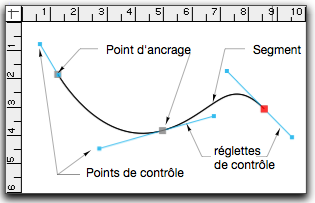
\includegraphics[width = 1\textwidth]{Bezier.png}
  \caption{courbe de Bézier}
  
\end{figure}




\subsection{Objectif du projet }
Dans le cadre de ce projet, nous mettrons l'accent sur trois domaines clés : la conception, la fabrication et l'inspection de pièces et de produits industriels.

\subsubsection{Conception}
La géométrie joue un rôle central dans la conception de pièces et de produits industriels. Par exemple, les courbes de Bézier peuvent être utilisées pour définir les contours de pièces aérodynamiques, garantissant ainsi des performances optimales. De plus, les équations de surface permettent de décrire les formes complexes des pièces, facilitant ainsi leur modélisation et leur fabrication ultérieure.

\begin{figure}[H]
  \centering
  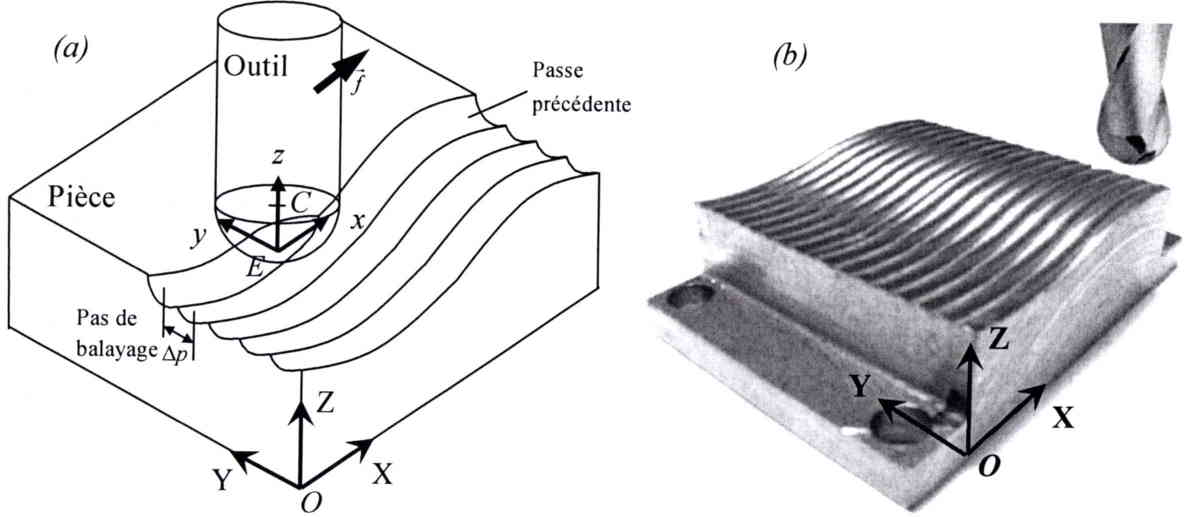
\includegraphics[width =\textwidth]{modelisation.png}
  \caption{exmple de modélisation à l'aide des équations de surface}
  
\end{figure}

\subsubsection{Fabrication}
La géométrie intervient également dans le processus de fabrication des composants industriels. Les formules mathématiques permettent de définir précisément les dimensions des pièces et les tolérances acceptables. Par exemple, l'utilisation de l'équation de la courbe involute pour les engrenages garantit un engagement correct et une transmission de puissance efficace.

\begin{figure}[H]
  \centering
  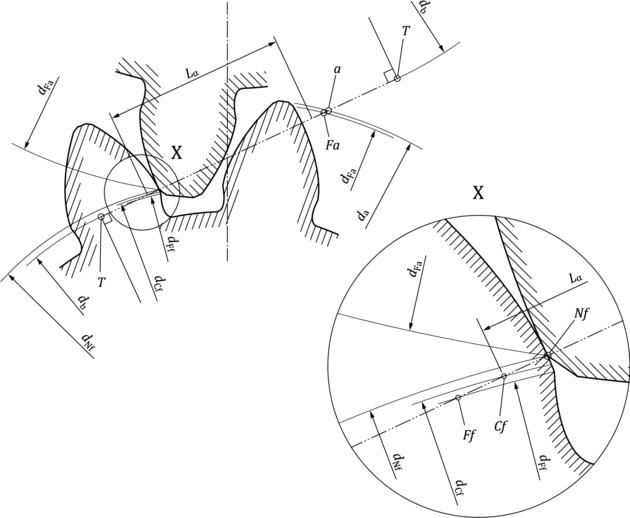
\includegraphics[width =\textwidth]{Tolerance.png}
  \caption{courbe involute pour les engrenages}
  
\end{figure}


\subsubsection{Inspection}
Enfin, la géométrie est essentielle lors de l'inspection des pièces fabriquées. Des méthodes de mesure précises basées sur des principes géométriques permettent de vérifier la conformité des pièces aux spécifications. Par exemple, la technique du bras de mesure avec capteurs à contact peut être utilisée pour inspecter la géométrie des pièces et détecter d'éventuelles déviations par rapport aux dimensions prévues.
\begin{figure}[H]
  \centering
  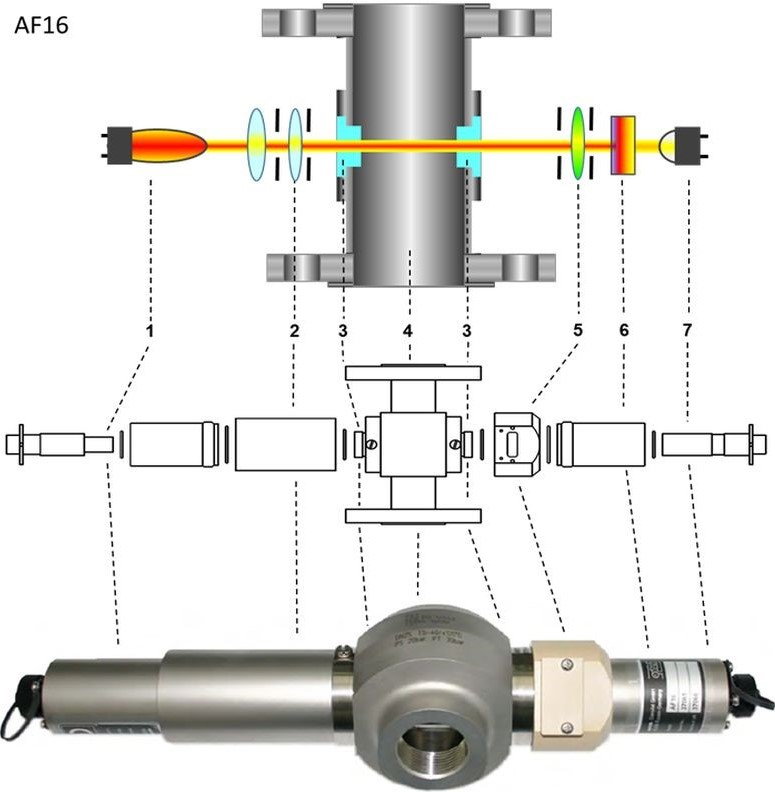
\includegraphics[width =\textwidth]{capteur.jpg}
  \caption{technique du bras de mesure avec capteurs à contact}
  
\end{figure}



\section{Fondements de la géométrie en ingénierie}

\subsection{Définition de la géométrie appliquée à l'ingénierie}
La géométrie appliquée à l'ingénierie est la branche des mathématiques qui étudie les propriétés et les relations des formes, des dimensions et des espaces dans le contexte de l'ingénierie. Elle fournit un cadre théorique et des outils pratiques pour la modélisation, la conception et l'analyse des objets et des systèmes techniques.

\subsection{Principaux concepts géométriques utilisés dans le domaine}
Dans le domaine de l'ingénierie, certains concepts géométriques fondamentaux sont largement utilisés. Parmi ceux-ci, on trouve :
\begin{itemize}
  \item Les points, les lignes et les plans : ces éléments de base sont utilisés pour définir les formes et les structures.

  \item Les dimensions : la géométrie permet de mesurer et de quantifier les dimensions des objets, telles que la longueur ($L$), la largeur ($W$) et la hauteur ($H$).

  \item Les angles : les angles sont essentiels pour décrire les orientations, les inclinaisons et les connexions entre les éléments. Par exemple, l'angle $\theta$ peut être utilisé pour décrire l'inclinaison d'un plan par rapport à un autre.

  \item Les courbes et les surfaces : les courbes (telles que les cercles et les courbes splines) et les surfaces (telles que les surfaces planes et les surfaces complexes) sont utilisées pour représenter et modéliser les formes tridimensionnelles. Par exemple, l'équation d'un cercle de rayon $r$ peut être donnée par $x^2 + y^2 = r^2$.

  \item Les transformations géométriques : les transformations géométriques, telles que les translations, les rotations et les homothéties, sont utilisées pour modifier et manipuler les formes. Par exemple, une translation d'un vecteur $\mathbf{t} = (t_x, t_y, t_z)$ peut être représentée par les équations suivantes : $x' = x + t_x$, $y' = y + t_y$ et $z' = z + t_z$.
\end{itemize}

\subsection{Exemples concrets de l'application de la géométrie dans différents domaines de l'ingénierie}
La géométrie est appliquée dans de nombreux domaines de l'ingénierie, notamment :
\begin{itemize}
  \item Mécanique : la géométrie est utilisée pour concevoir des pièces et des mécanismes, analyser les contraintes et les déformations, et optimiser les structures. Par exemple, l'équation du moment fléchissant $M(x)$ dans une poutre peut être donnée par $M(x) = -E \cdot I \cdot \frac{d^2w}{dx^2}$, où $E$ est le module d'élasticité, $I$ est le moment quadratique de la section transversale et $w(x)$ est la déformation de la p

  \item Aérospatiale : la géométrie est utilisée pour modéliser et simuler les aéronefs, les fusées et les satellites, et pour planifier les trajectoires et les mouvements. Par exemple, l'équation des trajectoires balistiques peut être donnée par les équations de mouvement : $x(t) = x_0 + v_{0x} \cdot t$, $y(t) = y_0 + v_{0y} \cdot t - \frac{1}{2} \cdot g \cdot t^2$, où $(x_0, y_0)$ sont les coordonnées initiales, $(v_{0x}, v_{0y})$ sont les composantes initiales de la vitesse et $g$ est l'accélération gravitationnelle.

  \item Électronique : la géométrie est utilisée pour concevoir et modéliser les circuits imprimés, les composants électroniques et les agencements spatiaux des systèmes électroniques. Par exemple, l'équation de la résistance d'un fil conducteur de longueur $L$ et de section transversale $A$ peut être donnée par $R = \rho \cdot \frac{L}{A}$, où $\rho$ est la résistivité du matériau.

  \item Architecture : la géométrie est utilisée pour concevoir les plans et les formes des bâtiments, créer des structures esthétiques et fonctionnelles, et optimiser l'utilisation de l'espace. Par exemple, la forme d'un dôme peut être déterminée à l'aide d'une équation paramétrique, telle que $x(u,v) = r \cdot \sin(u) \cdot \cos(v)$, $y(u,v) = r \cdot \sin(u) \cdot \sin(v)$ et $z(u,v) = r \cdot \cos(u)$, où $(u,v)$ sont les paramètres et $r$ est le rayon du dôme.
\end{itemize}

\subsection{Importance de la précision géométrique dans la fabrication et l'assemblage des composants industriels}
La précision géométrique est cruciale dans la fabrication et l'assemblage des composants industriels. Des erreurs ou des écarts par rapport aux spécifications géométriques peuvent entraîner des problèmes de qualité, de compatibilité et de fonctionnalité. Par exemple, dans l'usinage d'une pièce avec des tolérances géométriques strictes, une erreur de positionnement ou une déformation de la forme peut compromettre l'ajustement et l'interchangeabilité des pièces.

Il est donc essentiel de prendre en compte la géométrie avec précision tout au long du processus de fabrication et d'assemblage, en utilisant des techniques de mesure et de contrôle dimensionnel pour garantir la conformité aux spécifications géométriques.




\section{Géométrie et conception}

\subsection{Présentation des logiciels de modélisation géométrique utilisés en ingénierie}
En ingénierie, il existe plusieurs logiciels de modélisation géométrique qui permettent de créer des représentations virtuelles précises des pièces et des produits industriels. Certains des logiciels couramment utilisés sont : 
\begin{itemize}

  \item AutoCAD : un logiciel de conception assistée par ordinateur (CAO) utilisé pour créer des dessins techniques en 2D et en 3D.

  \item SolidWorks : un logiciel de CAO 3D qui permet de modéliser, simuler et analyser des pièces et des assemblages.

  \item CATIA : un logiciel de CAO utilisé principalement dans l'industrie aérospatiale et automobile pour la conception de produits complexes.

  \item Siemens NX : un logiciel de CAO intégré qui offre des fonctionnalités de modélisation, d'analyse et de fabrication pour la conception de produits.
\end{itemize}

\subsection{Illustration de l'utilisation de la géométrie dans la conception de pièces et de produits industriels à l'aide d'exemples concrets}
La géométrie joue un rôle central dans la conception de pièces et de produits industriels. Par exemple, dans la conception d'un moteur, la géométrie est utilisée pour déterminer la forme des cylindres, des pistons et des soupapes, ainsi que pour optimiser les flux d'air et de carburant. Cette optimisation peut être réalisée en utilisant des équations telles que l'équation de Bernoulli :
\[ P + \frac{1}{2} \rho v^2 + \rho gh = \text{constante} \]
où \( P \) est la pression, \( \rho \) est la densité du fluide, \( v \) est la vitesse, \( g \) est l'accélération gravitationnelle et \( h \) est la hauteur. Dans la conception d'un circuit imprimé, la géométrie est utilisée pour positionner les composants électroniques et les pistes de connexion de manière précise et efficace.

\subsection{Explication des techniques de dimensionnement géométrique et de tolérancement utilisées pour garantir la qualité et l'interopérabilité des composants}
Le dimensionnement géométrique et le tolérancement sont des techniques essentielles utilisées en ingénierie pour spécifier les dimensions et les tolérances des composants. Le dimensionnement géométrique permet de définir les formes, les orientations, les positions et les tolérances requises pour assurer la fonctionnalité et l'assemblage correct des pièces. Par exemple, la tolérance de perpendicularité d'une pièce peut être spécifiée à l'aide de la formule :
\[ | \text{angle de déviation} | \leq \text{tolérance de perpendicularité} \]
Le tolérancement permet de spécifier les écarts admissibles par rapport aux dimensions idéales, garantissant ainsi l'interopérabilité des composants fabriqués par différents fournisseurs. Ces techniques utilisent des symboles et des annotations spécifiques, tels que les tolérances géométriques (par exemple, la circularité, la perpendicularité) et les tolérances dimensionnelles (par exemple, les tolérances de longueur, de diamètre).



\section{Explication des techniques de dimensionnement géométrique et de tolérancement utilisées pour garantir la qualité et l'interopérabilité des composants}

Le dimensionnement géométrique et le tolérancement sont des techniques essentielles utilisées en ingénierie pour spécifier les dimensions et les tolérances des composants. Le dimensionnement géométrique permet de définir les formes, les orientations, les positions et les tolérances requises pour assurer la fonctionnalité et l'assemblage correct des pièces. Par exemple, la tolérance de circularité d'un alésage peut être spécifiée à l'aide de la formule suivante :

\[
\text{{Tolérance de circularité}} = \text{{Diamètre maximum}} - \text{{Diamètre minimum}}
\]

Le tolérancement permet de spécifier les écarts admissibles par rapport aux dimensions idéales, garantissant ainsi l'interopérabilité des composants fabriqués par différents fournisseurs. Par exemple, une tolérance dimensionnelle de \(\pm 0.1 \, \text{{mm}}\) peut être spécifiée pour la longueur d'une pièce.

Ces techniques utilisent des symboles et des annotations spécifiques, tels que les tolérances géométriques (par exemple, la circularité, la perpendicularité) et les tolérances dimensionnelles (par exemple, les tolérances de longueur, de diamètre). Ces symboles et annotations sont régis par des normes internationales, telles que les normes ISO et ASME, pour assurer une compréhension et une communication claires entre les concepteurs, les fabricants et les inspecteurs.

En combinant le dimensionnement géométrique, le tolérancement et les logiciels de modélisation géométrique, les ingénieurs peuvent concevoir et fabriquer des composants et des produits de haute qualité, conformes aux spécifications et aux exigences de l'industrie.




\section{Géométrie et fabrication}

\subsection{Présentation des procédés de fabrication industrielle et de leur relation avec la géométrie}

Dans le domaine de l'ingénierie, différents procédés de fabrication industrielle sont utilisés pour transformer les matériaux bruts en pièces et produits finis. Ces procédés comprennent, entre autres, l'usinage, le moulage, le formage, l'assemblage et l'impression 3D. La géométrie joue un rôle crucial dans tous ces procédés, car elle détermine les formes, les dimensions et les caractéristiques des pièces fabriquées. La géométrie est utilisée pour définir les trajectoires d'usinage, les cavités de moulage, les outillages de formage, les gabarits d'assemblage, ainsi que les paramètres de fabrication nécessaires pour obtenir des produits conformes aux spécifications.

\subsection{Discussion sur l'importance de la géométrie dans la mise en place de processus de fabrication efficaces}

Une géométrie précise est essentielle pour garantir la qualité et l'efficacité des processus de fabrication. Une erreur ou une déviation géométrique peut entraîner des défauts de fabrication, des problèmes d'ajustement, des fuites, des dysfonctionnements ou une mauvaise performance des produits. La géométrie est utilisée pour définir les paramètres d'usinage, de moulage ou de formage, ainsi que pour déterminer les tolérances et les ajustements nécessaires. En optimisant la géométrie des pièces et des outillages, on peut réduire les temps de cycle, minimiser les rebuts, améliorer l'efficacité des processus de fabrication et garantir la conformité aux exigences du produit.

\subsection{Illustration de l'utilisation de la géométrie dans la programmation des machines-outils à commande numérique (CNC) pour obtenir des formes et des dimensions précises}

Les machines-outils à commande numérique (CNC) utilisent la géométrie pour programmer et contrôler les mouvements des outils de coupe. En utilisant des modèles géométriques 3D, les opérations de fraisage, de tournage ou de perçage peuvent être programmées avec précision. La géométrie permet de définir les trajectoires d'outil, les points d'usinage et les profondeurs de coupe pour obtenir des formes et des dimensions précises. Les logiciels de programmation CNC utilisent des formats de fichier, tels que le langage G-code, pour représenter et communiquer les informations géométriques nécessaires aux machines-outils. Grâce à l'utilisation de la géométrie, les pièces peuvent être fabriquées avec une grande précision, une répétabilité élevée et une meilleure efficacité des processus de fabrication.

Pour illustrer davantage l'utilisation de la géométrie dans la programmation CNC, voici quelques formules couramment utilisées :

\begin{itemize}
  \item Trajectoire d'outil pour le fraisage : $x = x_0 + R\cos(\theta)$, $y = y_0 + R\sin(\theta)$, où $x_0$ et $y_0$ représentent les coordonnées de l'origine, $R$ est le rayon de l'outil et $\theta$ est l'angle de rotation.

  \item Vitesse d'avance : $F = \frac{N}{T}$, où $F$ est la vitesse d'avance, $N$ est le nombre de tours par minute de la broche et $T$ est le nombre de dents de l'outil.

  \item Profondeur de coupe : $D = d - z$, où $D$ est la profondeur de coupe, $d$ est la profondeur totale de la pièce et $z$ est la profondeur de la passe.

\end{itemize}

Ces formules permettent de calculer les paramètres nécessaires pour programmer les machines-outils CNC et obtenir des formes et des dimensions précises lors de la fabrication des pièces.

En utilisant la géométrie et ces formules dans la programmation CNC, les ingénieurs peuvent optimiser les processus de fabrication, réduire les erreurs et obtenir des produits de haute qualité conformes aux spécifications géométriques requises.


\section{Conclusion}

\subsection{Récapitulation des points clés soulignant l'importance de la géométrie en ingénierie}

La géométrie joue un rôle essentiel dans le domaine de l'ingénierie. Elle est utilisée dans la conception, la fabrication et l'inspection de pièces et de produits industriels. La précision géométrique est cruciale pour garantir la qualité, la fonctionnalité et l'interopérabilité des composants. La géométrie permet de définir les formes, les dimensions, les tolérances et les caractéristiques géométriques nécessaires à la réalisation de produits conformes aux exigences spécifiées. Elle est également utilisée dans la programmation des machines-outils et dans les techniques d'inspection pour assurer la conformité des pièces fabriquées. En résumé, la géométrie est un pilier fondamental de l'ingénierie, contribuant à l'efficacité, à la qualité et à l'innovation dans de nombreux domaines industriels.

La précision géométrique peut être exprimée mathématiquement par des formules telles que :
\begin{itemize}
  \item La distance entre deux points dans l'espace tridimensionnel : $d=\sqrt{(x_2-x_1)^2+(y_2-y_1)^2+(z_2-z_1)^2}$

  \item L'angle entre deux vecteurs : $\cos(\theta) = \frac{\vec{a}\cdot\vec{b}}{|\vec{a}||\vec{b}|}$

  \item La surface d'un objet : $A = \iint_S dS$, où $S$ est la surface de l'objet

  \item Le volume d'un objet : $V = \iiint_V dV$, où $V$ est le volume de l'objet.

\end{itemize}

\subsection{Réflexion personnelle sur les apprentissages tirés du projet}
Travailler sur ce projet m'a permis de prendre conscience de l'importance de la géométrie dans le domaine de l'ingénierie. J'ai réalisé combien la précision géométrique influence directement la qualité des produits et des processus de fabrication. J'ai également compris comment les logiciels de modélisation géométrique, les techniques de dimensionnement et les technologies d'inspection basées sur la géométrie sont des outils précieux pour les ingénieurs. Ce projet m'a également donné l'occasion d'approfondir mes connaissances en matière de conception, de fabrication et d'inspection dans le domaine de l'ingénierie.








\end{document}


